\section{\Acrfull{bsj} detection}

For detection of \gls{bsj}s, I used the five tools already introduced in
\cref{subsec:circrna_detection}.
As shown in \cref{fig:detection_bars}, find\_circ, CIRI2, DCC, and
circexplorer2 detect a similar number of \gls{bsj}s, while segemehl detects
almost ten times as many \gls{bsj}s as its closest competitor, DCC.

\begin{figure}[ht] \centering

    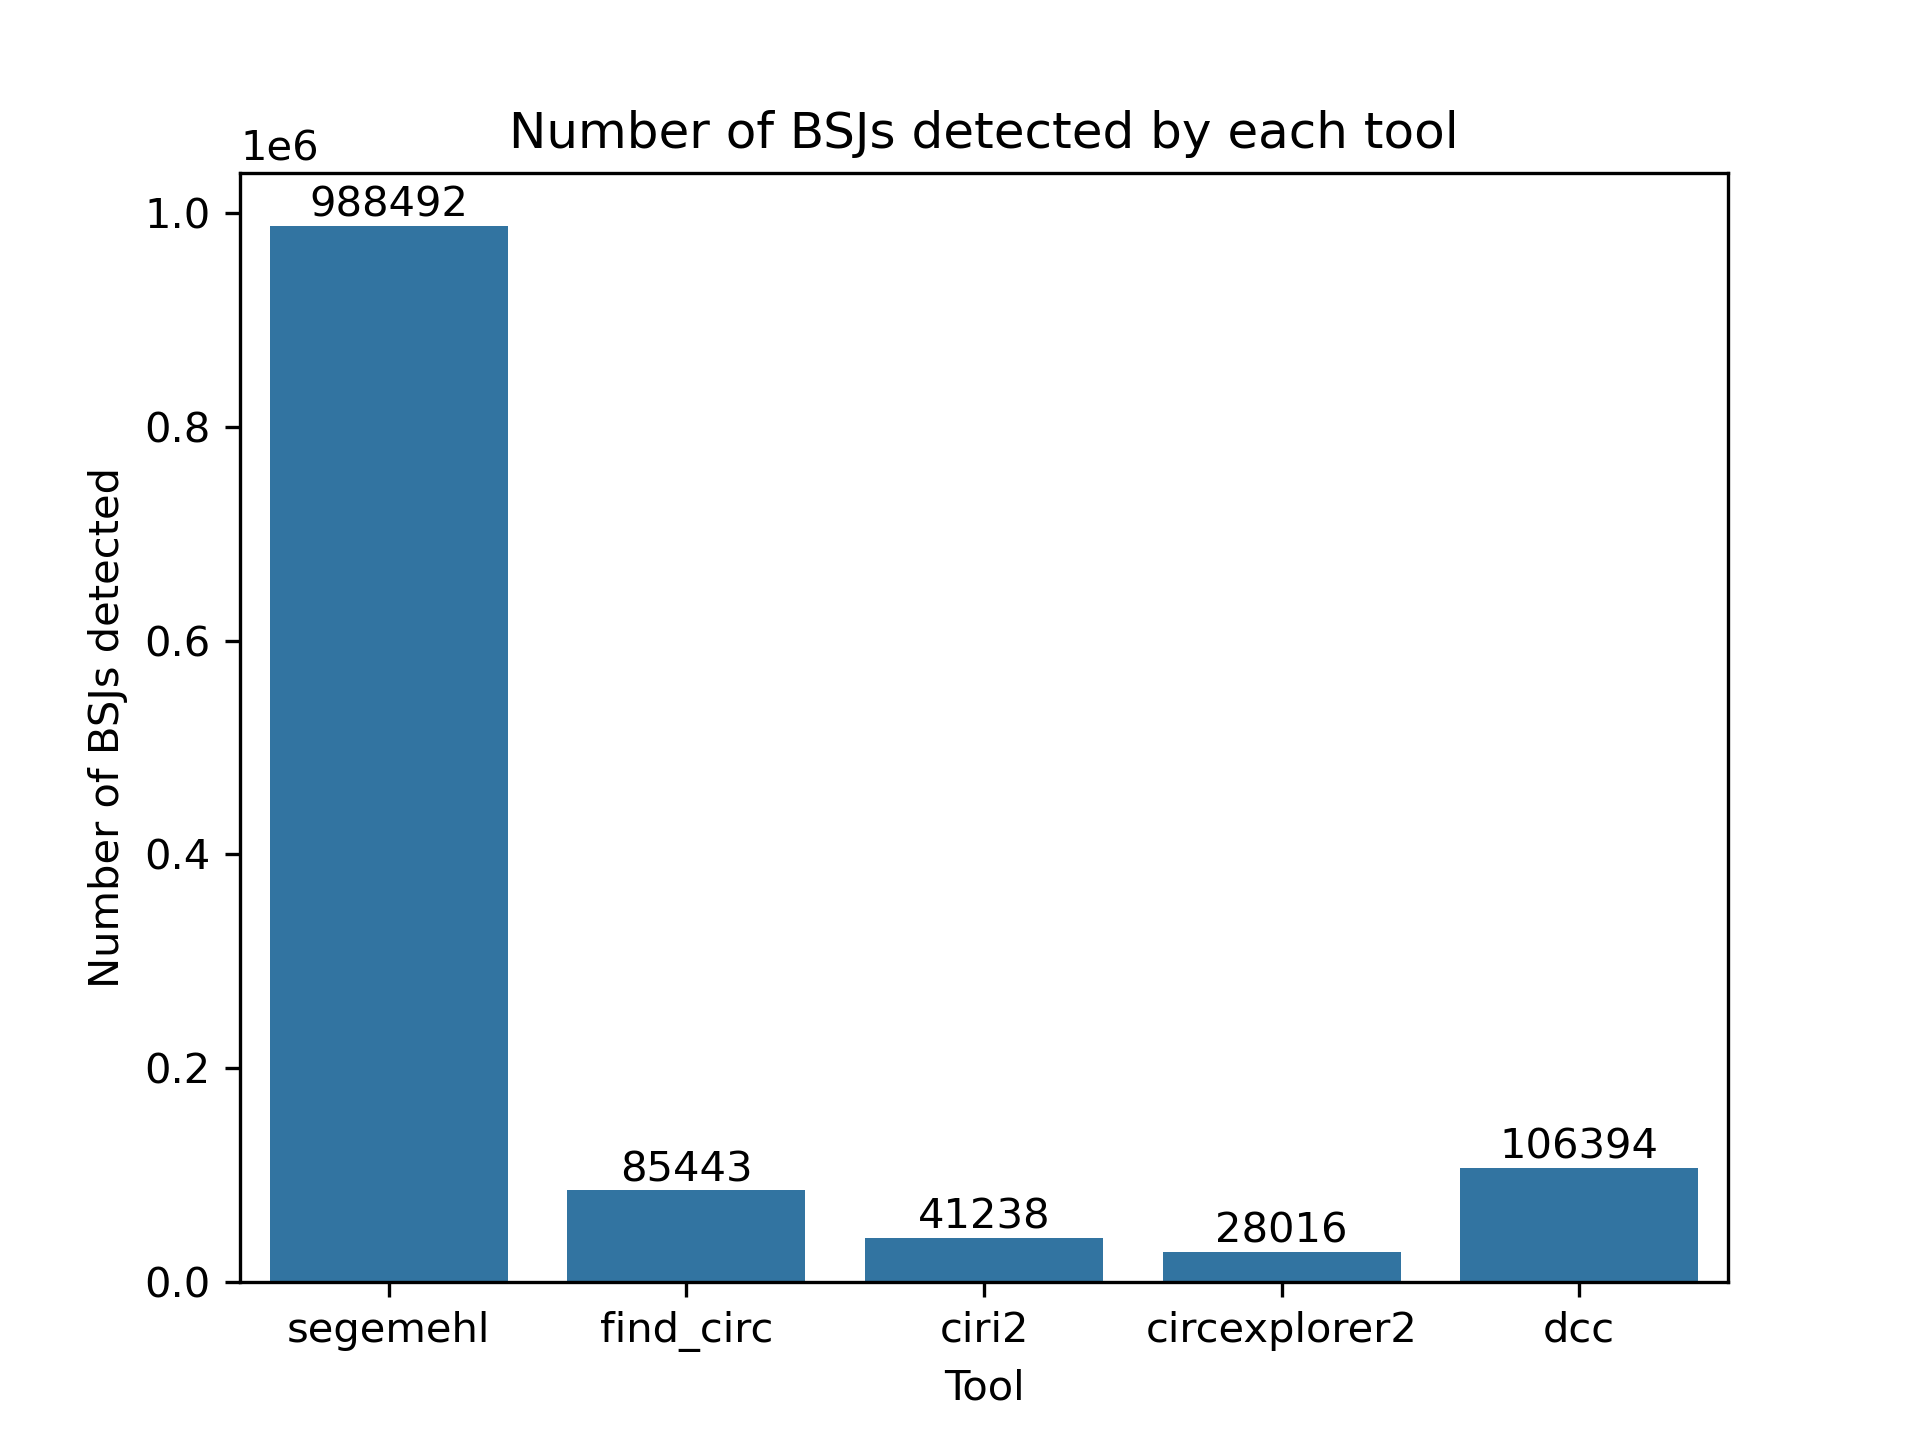
\includegraphics[width=0.7\textwidth]{chapters/4_results_and_discussion/figures/detection/n_bsjs_detected.png}
    \caption{Number of \gls{bsj}s detected by each tool.
        While find\_circ, CIRI2, DCC and circexplorer2 detect a similar number of
        \gls{bsj}s, segemehl detects a much larger number of \gls{bsj}s.
    }
    \label{fig:detection_bars}
\end{figure}
Similar behavior was previously observed by \textcite{zeng_comprehensive_2017},
where segemehl was among the top performers in terms of sensitivity, but also
had a high false positive rate.
The lowest numbers of \gls{bsj}s were detected by circexplorer2 and CIRI2,
which both have built-in filters to reduce false
positives\supercite{zhang_diverse_2016,gao_circular_2018}.

\subsection{Agreement between tools}

To assess the agreement between the tools, I used UpSet plots, which show the
overlap of \gls{bsj}s detected by different tools.
When identifying the overlap between tools, the most strict approach is to
consider only \gls{bsj}s with identical start and end positions and on the same
strand as the same \gls{bsj}.
The according plot is shown in \cref{fig:detection_upset_0_strand}.
While there are a total of x \gls{bsj}s detected by at least two tools, only y
\gls{bsj}s are detected by three tools, and none are detected by four or five
tools.

When ignoring the strand information, the number of \gls{bsj}s detected by
three tools increases substantially, as shown in
\cref{fig:detection_upset_0_nostrand}.
Also the number of \gls{bsj}s detected by two tools increases, while still no
\gls{bsj}s are detected by four or five tools.

Allowing a shift of 1 bp in the start and end positions while ignoring the
strand information changes the results drastically.
As shown in \cref{fig:detection_upset_1_nostrand}, a large number of \gls{bsj}s
are detected by four and even five tools.

As shown in \cref{fig:detection_upset_1_strand}, allowing a shift of 1 bp while
considering the strand information also leads to a number of \gls{bsj}s
detected by four and five tools, but the number is way lower than when ignoring
the strand information.

Increasing the allowed shift to larger values, e.g., 20 bp, does not lead to a
substantial change compared to the results when allowing a shift of 1 bp, as
shown in \cref{fig:detection_upset_20_nostrand}.

\begin{figure}[ht] \begin{tabular}{cc} \begin{subfigure}{.5\textwidth}
                                           \centering

                                           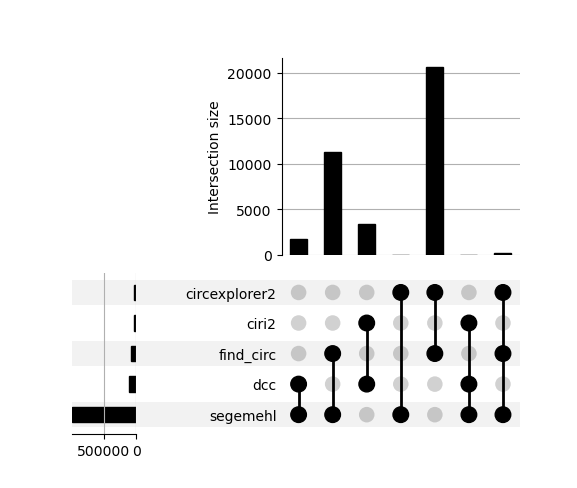
\includegraphics[width=\linewidth]{chapters/4_results_and_discussion/figures/detection/upset/diff_0_strand.png}
                                           \caption{No shift allowed, strand
                                               considered}
                                           \label{fig:detection_upset_0_strand}
                                       \end{subfigure} &
               \begin{subfigure}{.5\textwidth} \centering

                       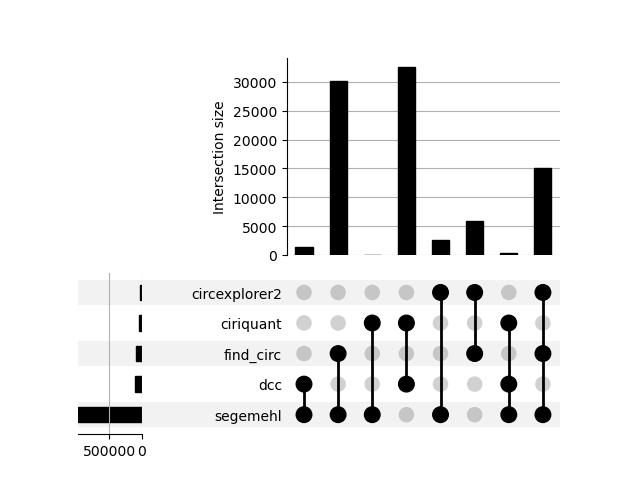
\includegraphics[width=\linewidth]{chapters/4_results_and_discussion/figures/detection/upset/diff_0_nostrand.png}
                       \caption{No shift allowed, strand ignored}
                       \label{fig:detection_upset_0_nostrand} \end{subfigure}
               \\ \multicolumn{2}{c}{
                   \begin{subfigure}{\textwidth} \centering

                           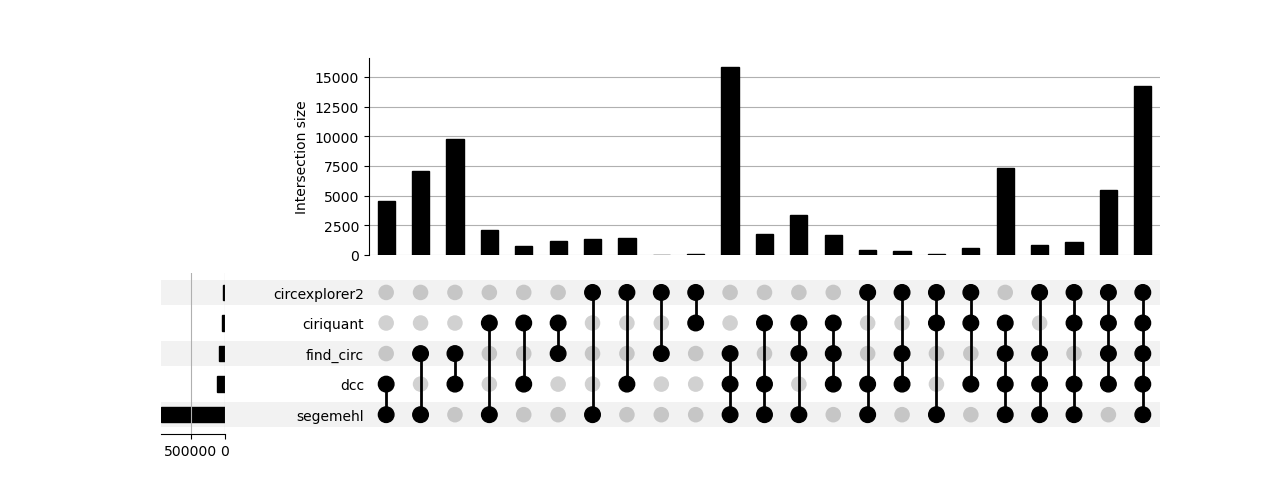
\includegraphics[width=\linewidth]{chapters/4_results_and_discussion/figures/detection/upset/diff_1_nostrand.png}
                           \caption{Shift of 1 allowed, strand ignored}
                           \label{fig:detection_upset_1_nostrand}

                       \end{subfigure}}\end{tabular} \caption{Upset plots
        showing the overlap of
        \gls{bsj}s detected by different tools using various grouping criteria.
        Only groups with at least two agreeing tools are displayed.
        When considering strand information and only counting \gls{bsj}s with identical
        start and end positions, many \gls{bsj}s are detected by just two tools, with
        very few detected by three tools (\cref{fig:detection_upset_0_strand}).
        Ignoring the strand information substantially increases the number of
        \gls{bsj}s detected by 3 tools (\cref{fig:detection_upset_0_nostrand}).
        Allowing a shift of 1 bp in the start and end positions while ignoring the
        strand information changes the results drastically, leading to a large number
        of \gls{crna}s with agreement between 4 and even 5 tools
        (\cref{fig:detection_upset_1_nostrand}).
    }
    \label{fig:detection_upset}
\end{figure}

\begin{figure}[ht]
    \centering

    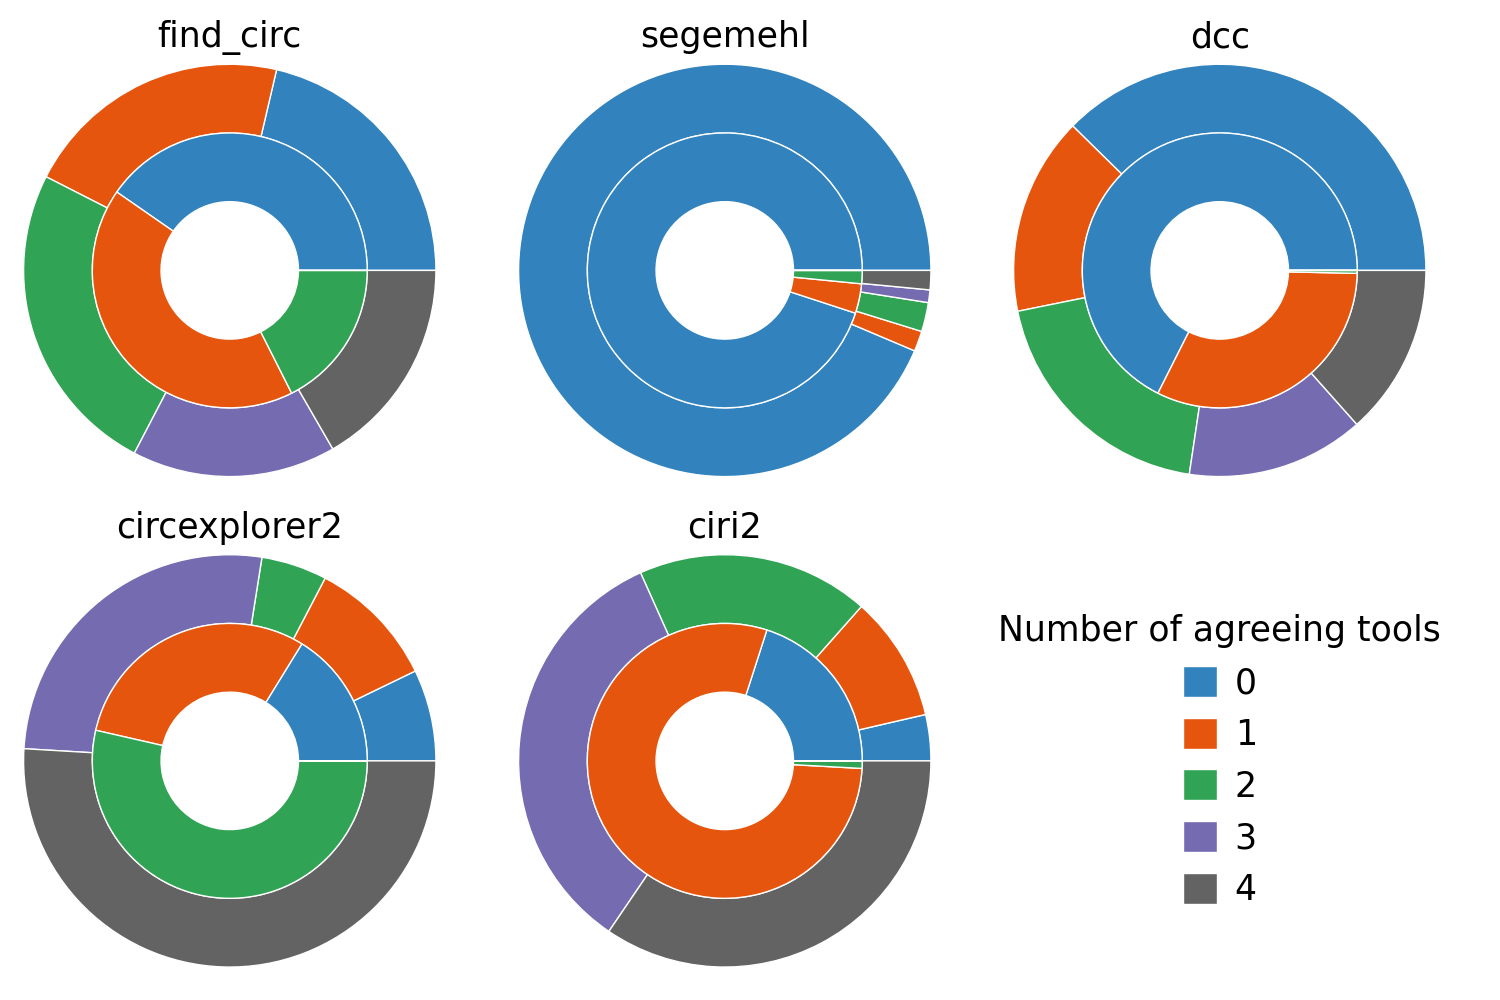
\includegraphics[width=0.7\textwidth]{chapters/4_results_and_discussion/figures/detection/pies.png}
    \caption{Pie charts showing the agreement of each tool with the others.
        The inner circle shows the agreement without allowing a shift in the start and
        end positions, while the outer circle shows the agreement when allowing a shift
        of 1 bp.
        While find\_circ, dcc, circexplorer2, and ciriquant behave similarly, segemehl
        detects a much larger number of \gls{bsj}s, with a large portion of them not
        being detected by any other tool.
    }
    \label{fig:detection_pies}
\end{figure}

\begin{figure}[ht]
    \begin{tabular}{cc}
        \begin{subfigure}{.4\textwidth}
            \centering

            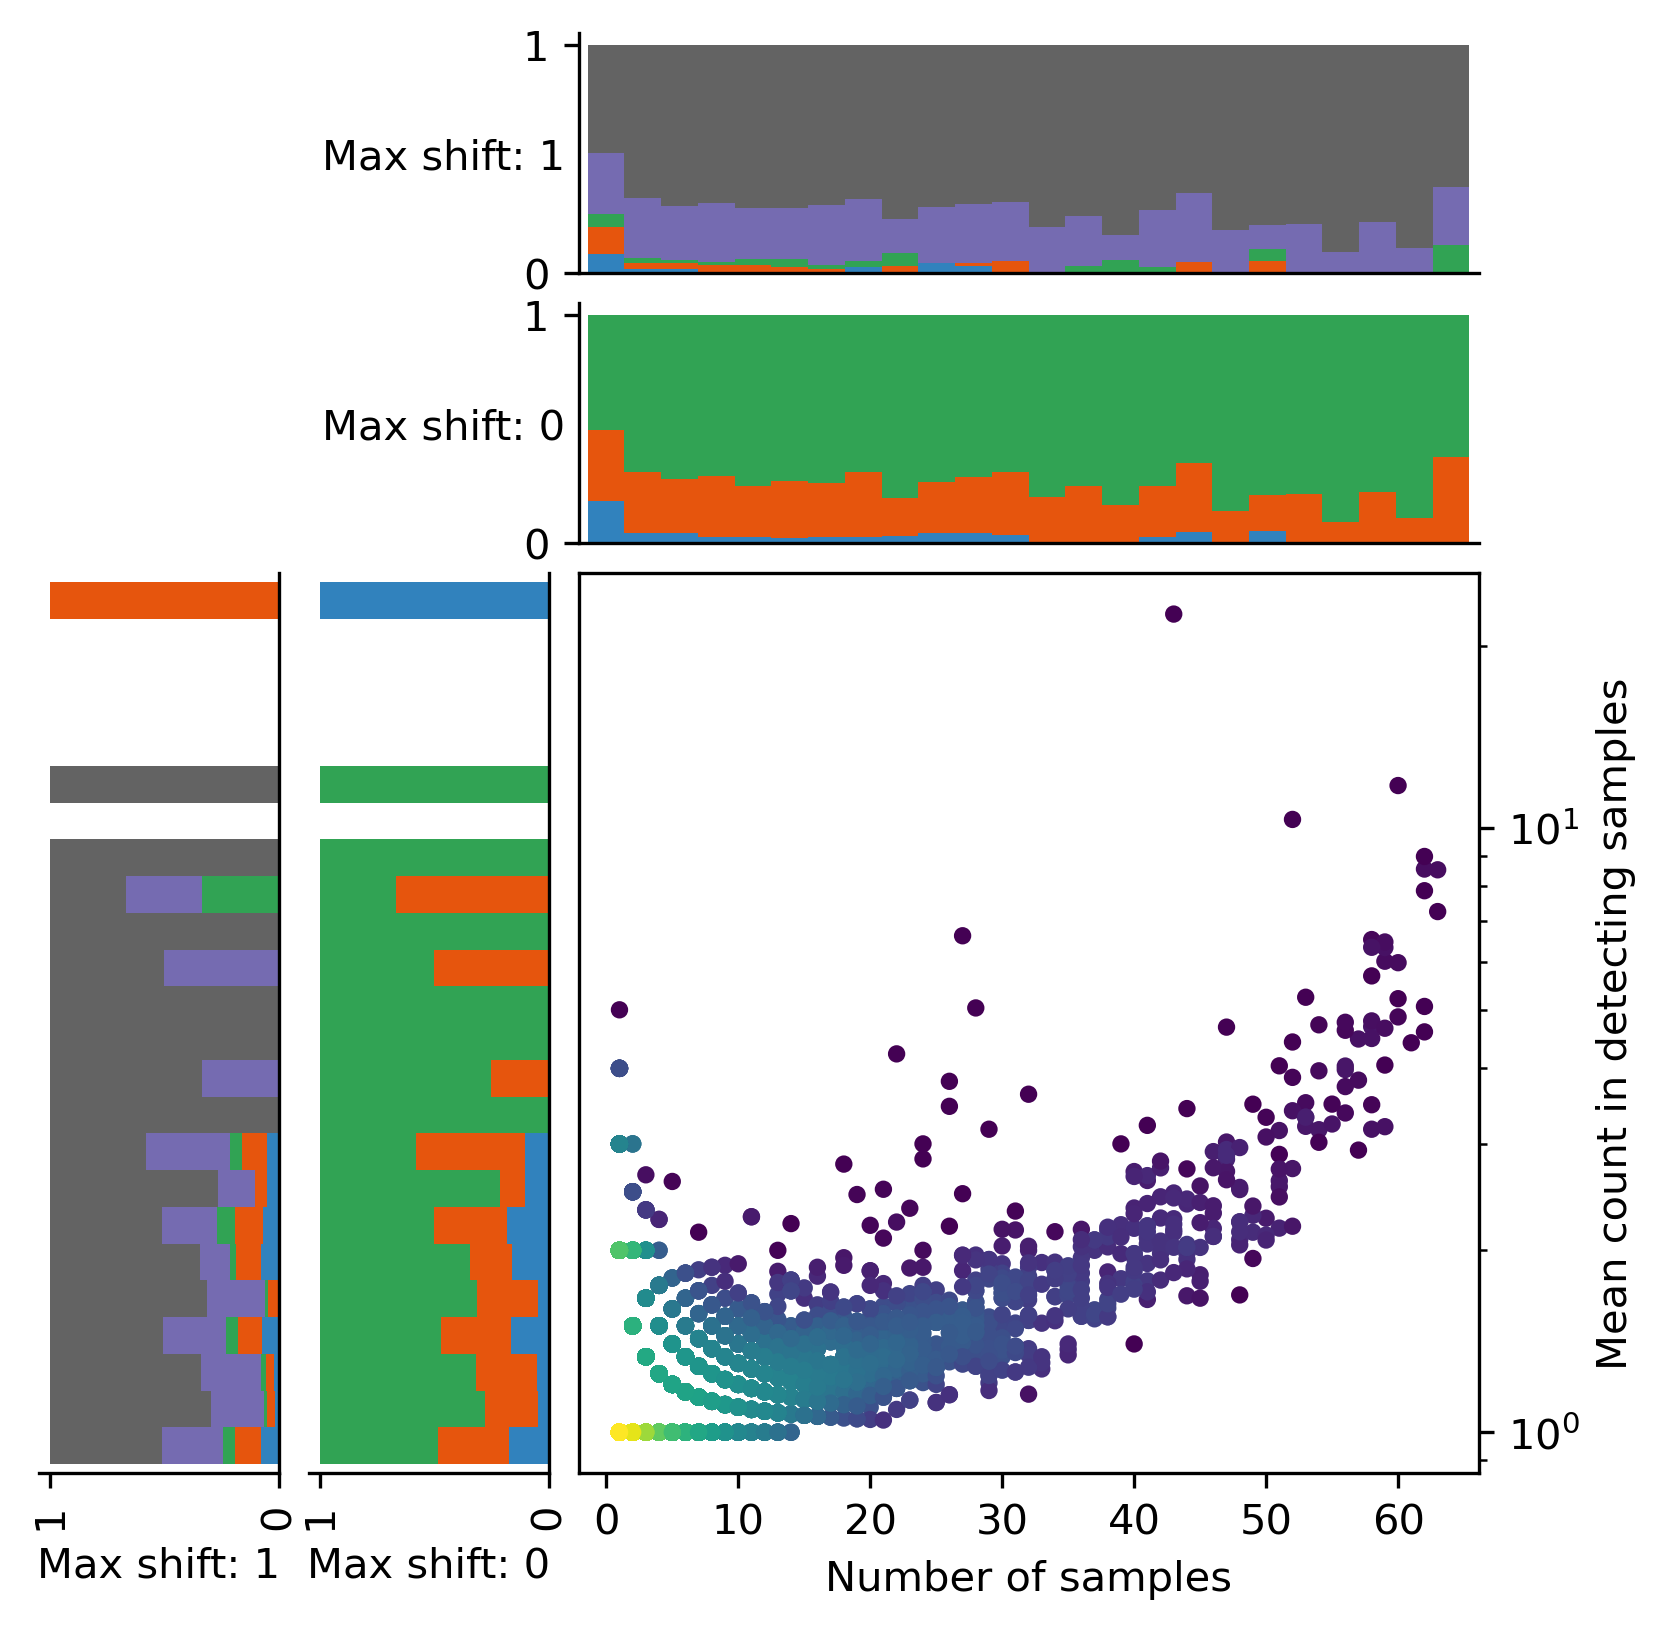
\includegraphics[width=\linewidth]{chapters/4_results_and_discussion/figures/detection/density/circexplorer2.png}
            \caption{CircExplorer2}
            \label{fig:detection_density_circexplorer2}
        \end{subfigure}
         &
        \begin{subfigure}{.4\textwidth}
            \centering

            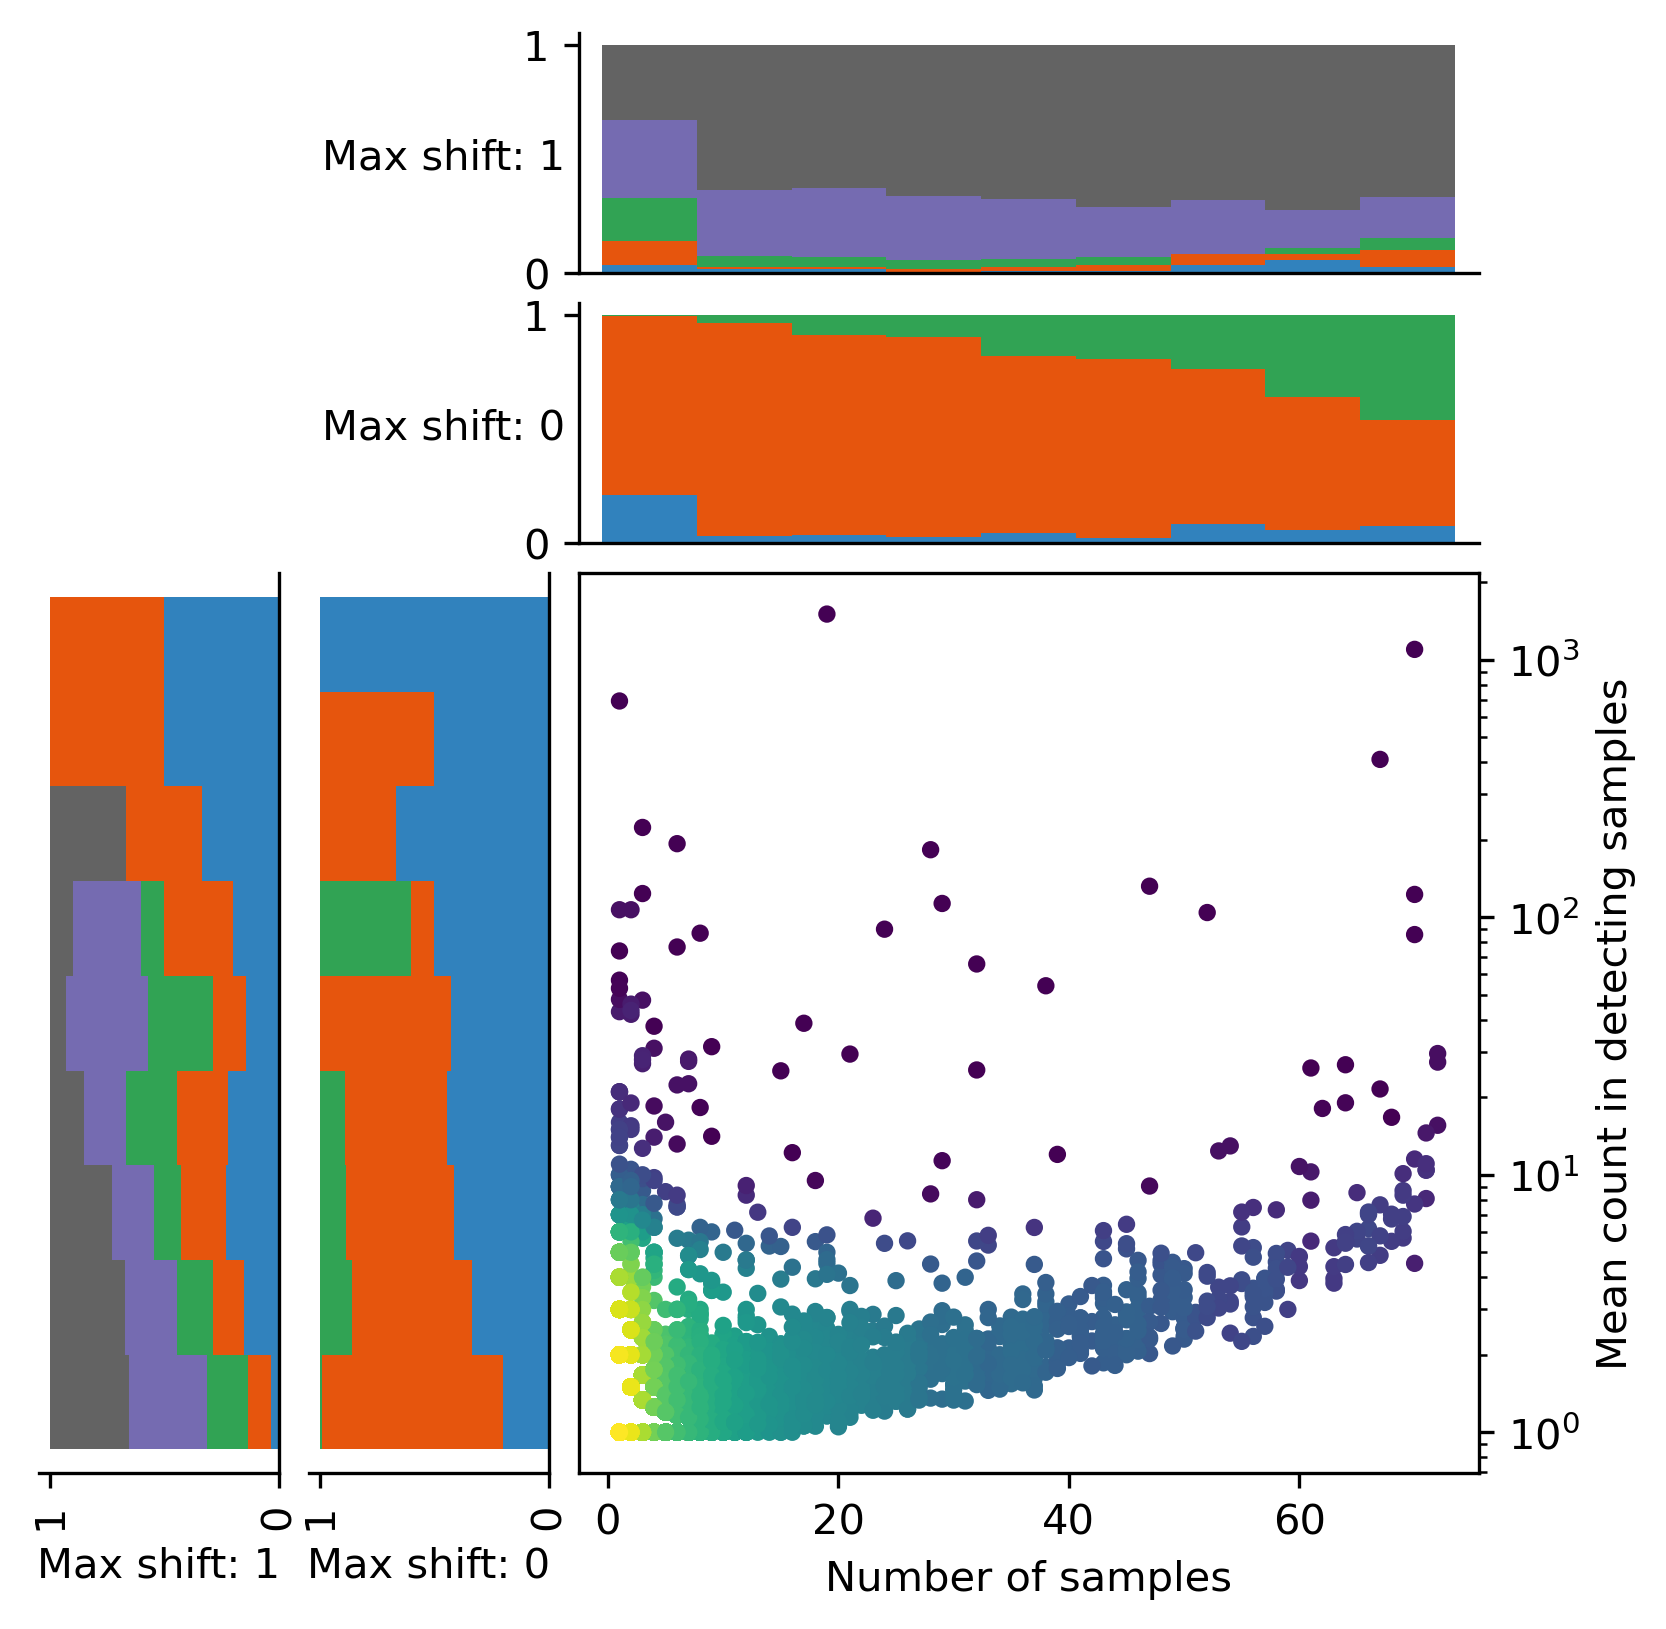
\includegraphics[width=\linewidth]{chapters/4_results_and_discussion/figures/detection/density/ciri2.png}
            \caption{CIRI2}
            \label{fig:detection_density_ciri2}
        \end{subfigure}     \\
        \begin{subfigure}{.4\textwidth}
            \centering

            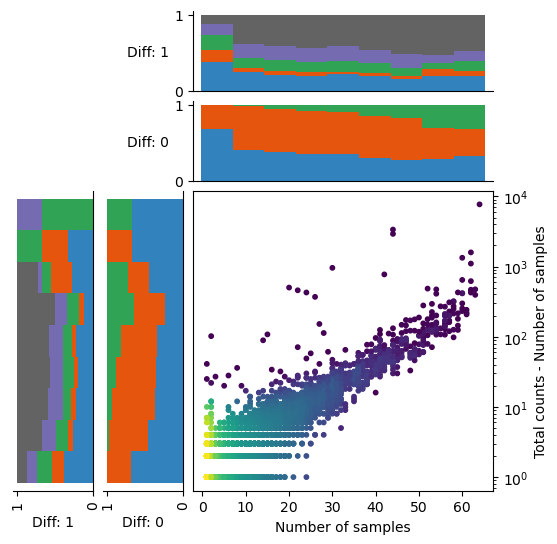
\includegraphics[width=\linewidth]{chapters/4_results_and_discussion/figures/detection/density/dcc.png}
            \caption{DCC}
            \label{fig:detection_density_dcc}
        \end{subfigure}
         &
        \begin{subfigure}{.4\textwidth}
            \centering

            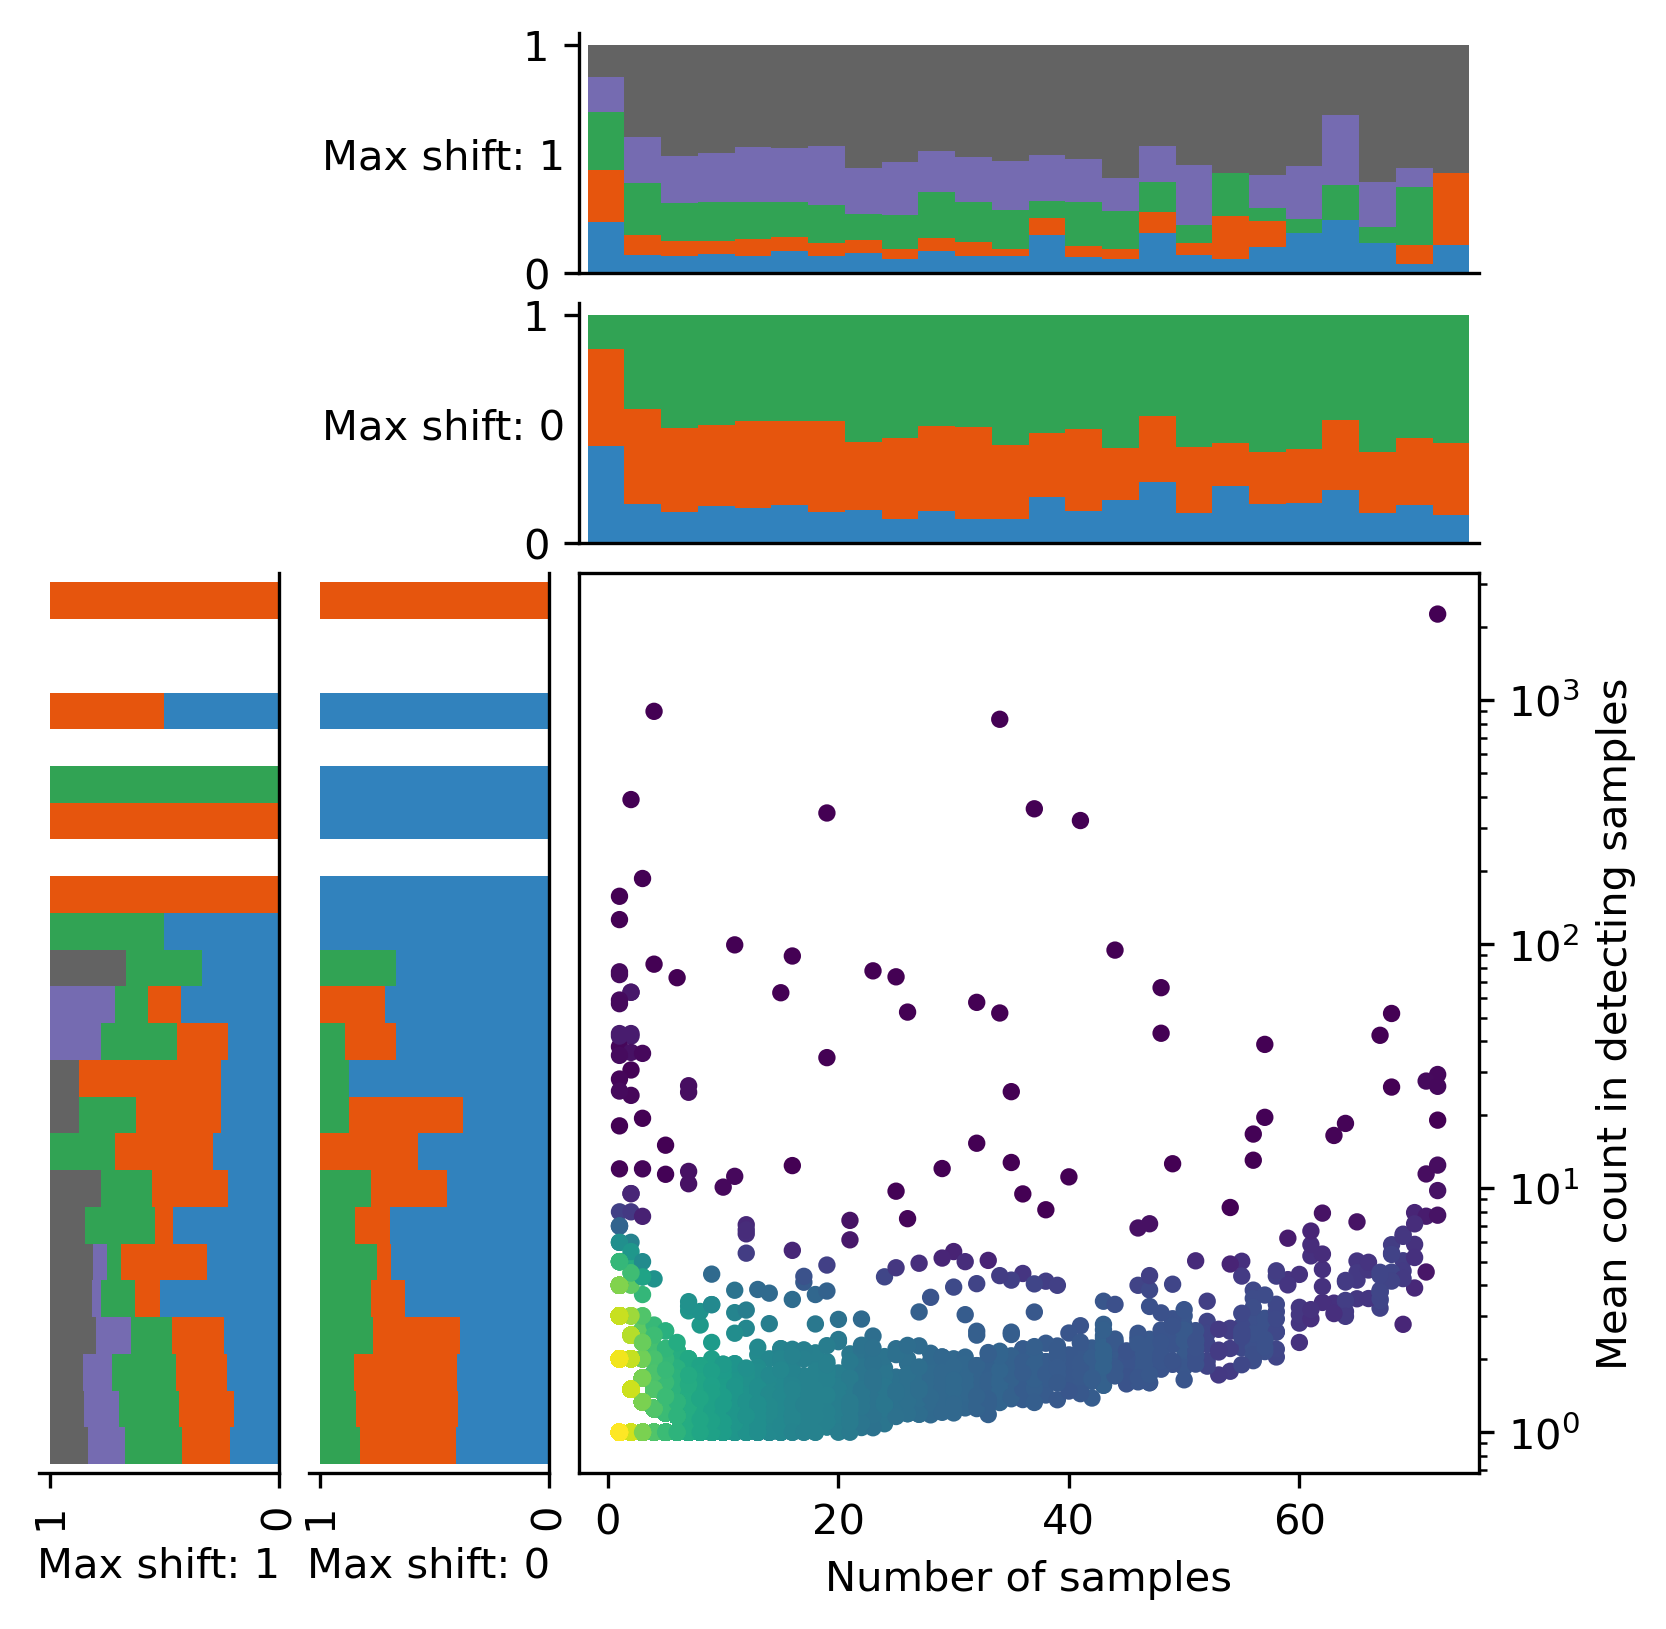
\includegraphics[width=\linewidth]{chapters/4_results_and_discussion/figures/detection/density/find_circ.png}
            \caption{find\_circ}
            \label{fig:detection_density_find-circ}
        \end{subfigure} \\
        \begin{subfigure}{.4\textwidth}
            \centering

            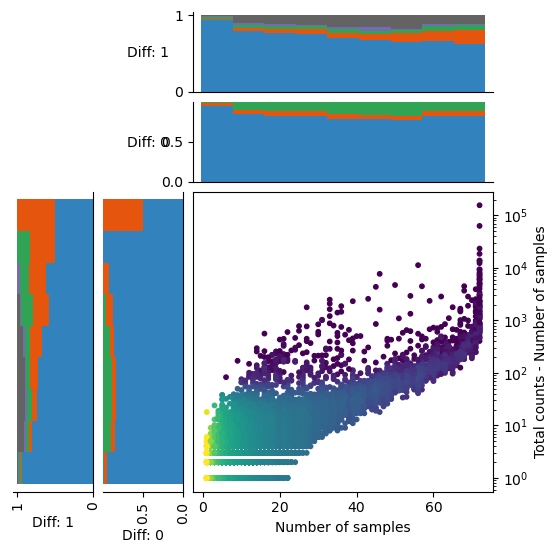
\includegraphics[width=\linewidth]{chapters/4_results_and_discussion/figures/detection/density/segemehl.png}
            \caption{Segemehl}
            \label{fig:detection_density_segemehl}
        \end{subfigure}
         &
        \begin{subfigure}{.4\textwidth}
            \centering
            % TODO: Add legend
            %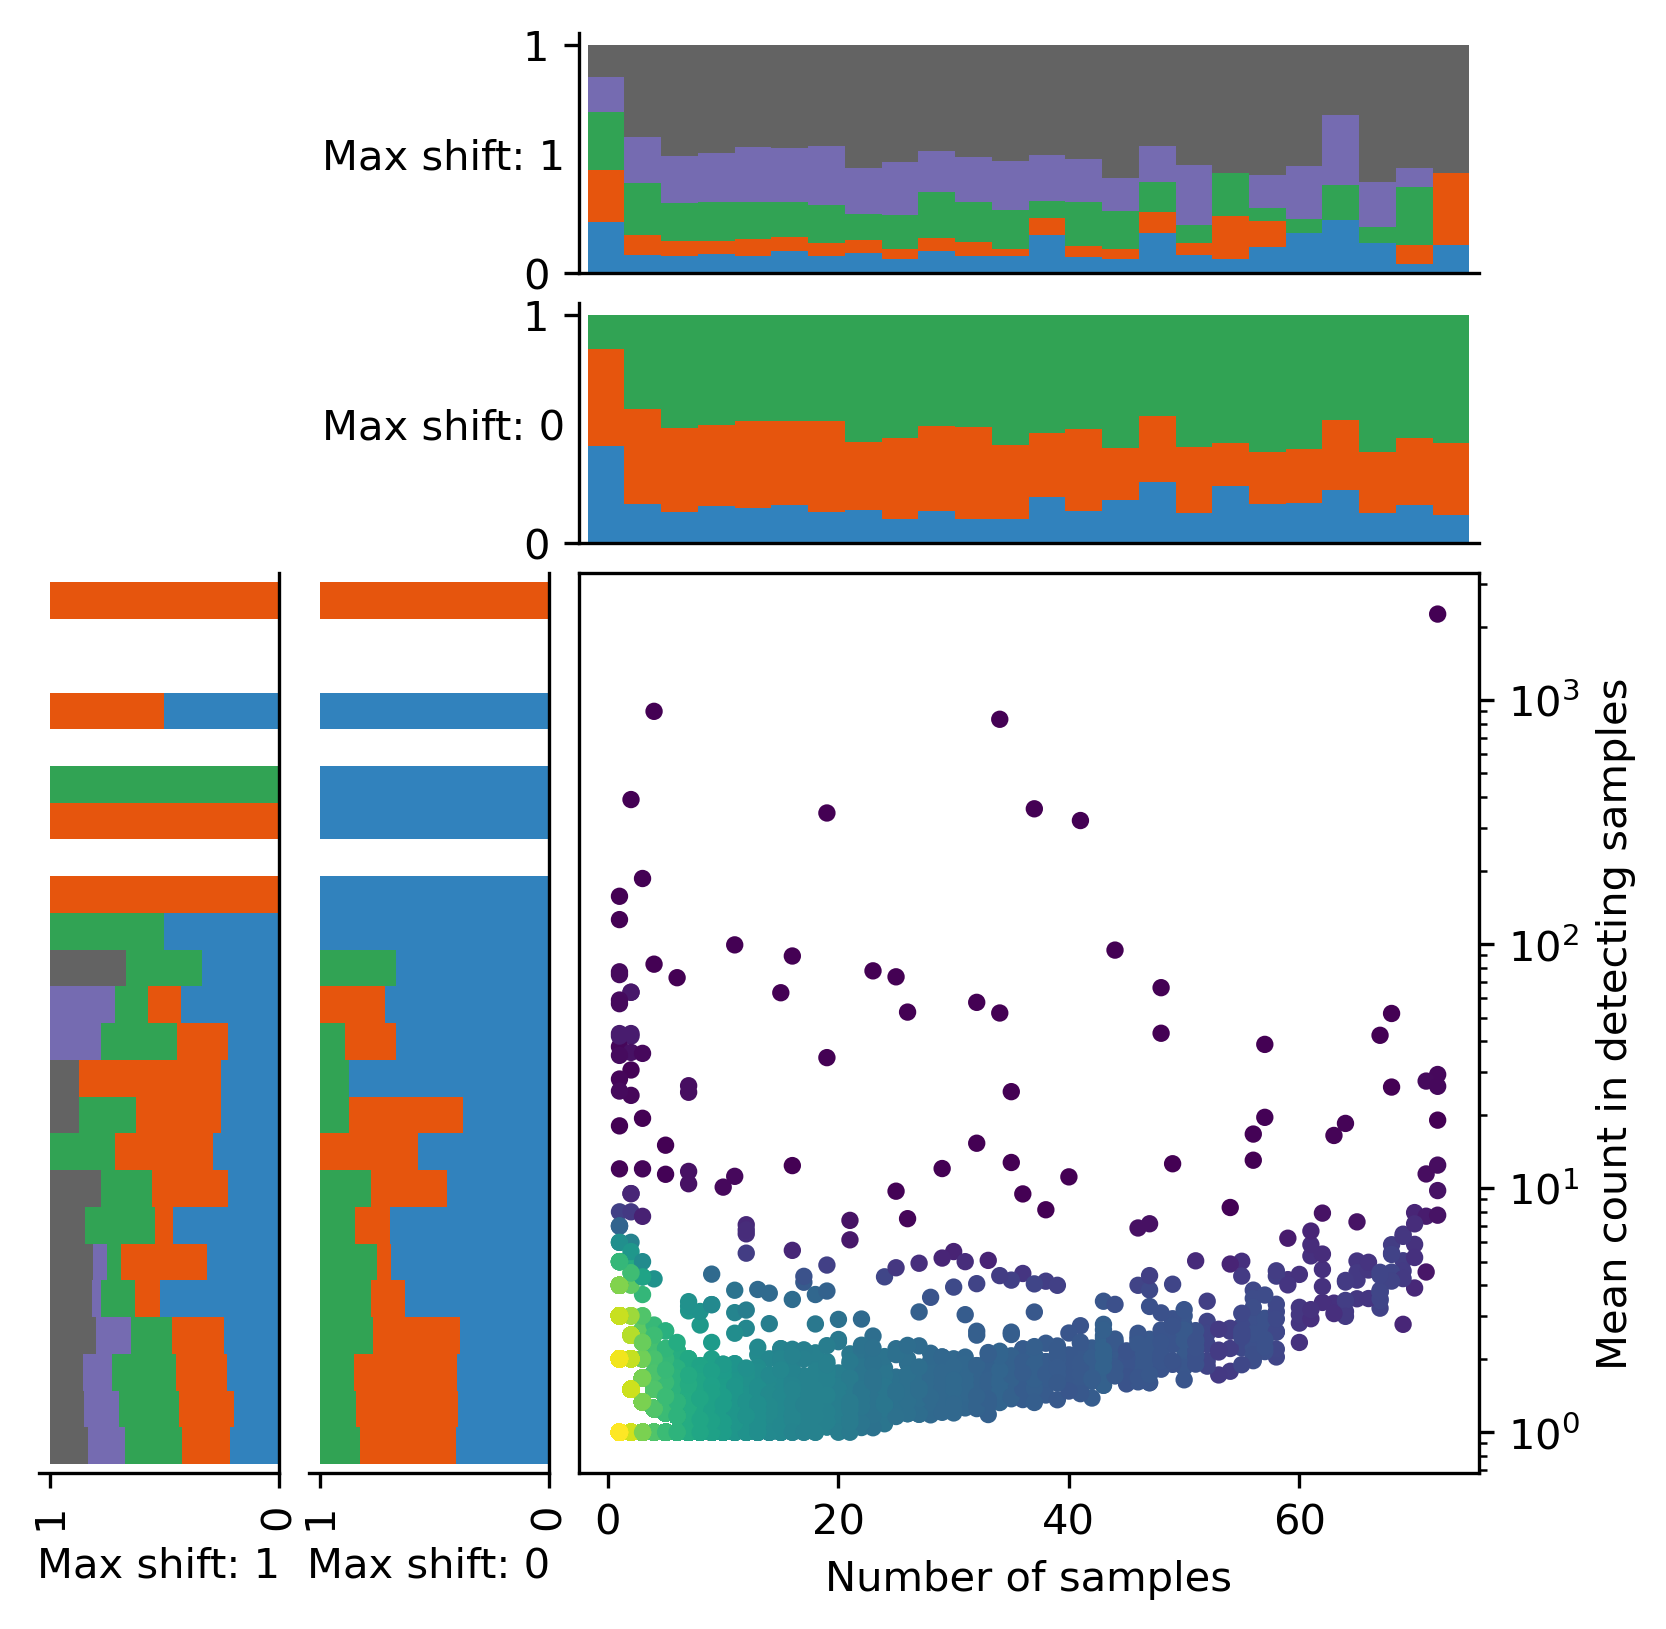
\includegraphics[width=\linewidth]{chapters/4_results_and_discussion/figures/detection/density/find_circ.png}
            \caption{Legend}
        \end{subfigure}
    \end{tabular}
    \caption{Distributions of \gls{bsj}s detected by each tool.
        The x-axis shows the number of tools that detected a \gls{bsj}, while the
        y-axis shows the logarithm of the number of reads supporting the \gls{bsj}
        across all samples.
        The color indicates the density of \gls{bsj}s at a given point.
        The stacked bar plots above and left of the scatter plots show the number of
        agreeing tools in the respective slice.
    }
    \label{fig:detection_density}
\end{figure}
